% Chapter Template

\chapter{Design and Implementation} % Main chapter title

\label{Chapter2} % Change X to a consecutive number; for referencing this chapter elsewhere, use \ref{ChapterX}

%\lhead{Chapter 2. \emph{Design and Implementation}} % Change X to a consecutive number; this is for the header on each page - perhaps a shortened title
\fancyhead[RO]{\thepage}
\fancyhead[RE]{\thepage}
\fancyhead[LE]{Chapter 2.~\emph{\Chaptername}}
\fancyhead[LO]{\emph{\ttitle}}
%----------------------------------------------------------------------------------------
%	SECTION 1
%----------------------------------------------------------------------------------------

\section{Modeling of a denser slab}

A denser slab having $\mu_r = 2\mu_o$ and $\epsilon_r = 2\epsilon_o$
is simulated to test the results and accuracy of our algorithm. these results will be compared with
results of NIM slab.

%-----------------------------------
%	SUBSECTION 1.1
%-----------------------------------
\subsection{Finite Difference Time Domain (FDTD) technique}
FDTD method is used to solve problems related to electromagnetic. It is very easy to implement but require much computational power and time as this is a recursive technique. The main benefit of using this technique is that it is accurate on wide range of frequency. 

Maxwell's equations (Ampere's and Faraday's laws) can be written as finite differences using FDTD. A function $f(x)$ whose value need to be found at $x_o$ is given by %ref here
	\begin{equation}
	\left. \frac {df(x)}{d(x)}\right|_{x=x_o} \approx 
	\frac {f \left( x_o + \frac{\delta}{2} \right) - f \left( x_o - \frac{\delta}{2} \right) }{\delta}
	\end{equation}
this equation provides an approximation of derivative of $f(x)$ at $x_o$ but the function is sampled at an offset $\delta$ from the original point $x_o$. It have second-order accuracy or second-order behavior. This implies if $\delta$ is reduced by a factor of 10 the error will be reduced by 100. if $\delta = 0$ then $error = 0$.
%-----------------------------------
%	SUBSECTION 1.2
%-----------------------------------
\subsection{The Yee Algorithm}
Kane Yee proposed FDTD algorithm in 1966% ref here
. It can be summarized as follows:
\begin{enumerate}
\item Differential forms of Maxwell's equations are written with finite differences.
\item Solve the difference equations to get "update equations" that express the future value in terms of past value. Figure \ref{fig:fdtd}
\begin{figure}[htbp]
	\centering
		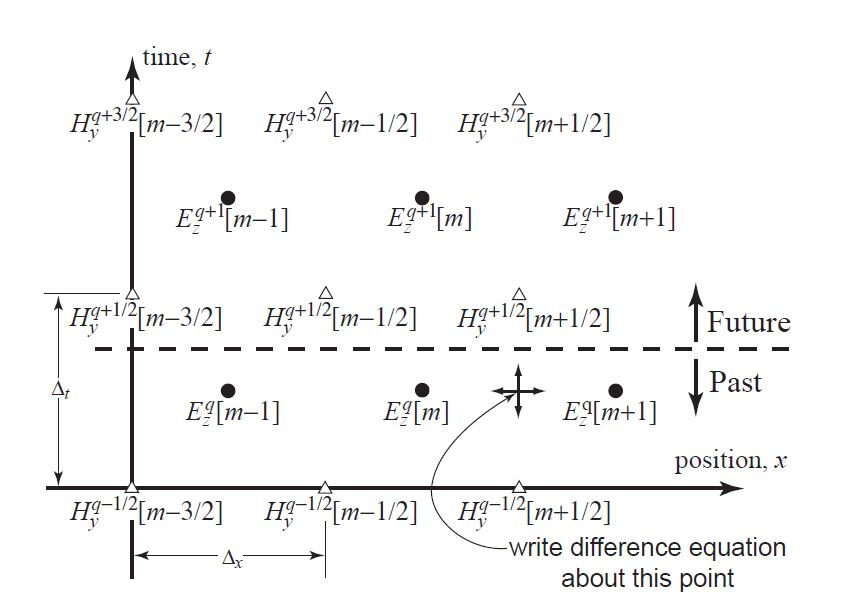
\includegraphics[width=4in]{Pictures/fdtd.jpg}
		%\rule{35em}{0.5pt}
	\caption[FDTD update equations]{Update equations at a point depend on past values of adjacent points.}
	\label{fig:fdtd}
\end{figure} 
\item Find the magnetic field component one time-step into the future for complete spatial domain. Using equation \eqref{eq:mag}
\begin{equation}
	H_y^{q+\frac {1}{2}} \left[ m + \frac {1}{2} \right] = H_y^{q-\frac {1}{2}} \left[ m + \frac {1}{2} \right]
+ \frac {\Delta_t}{\mu\Delta_x} \left( E_z^q \left[ m+1 \right] - E_z^q \left[m\right] \right)
\label{eq:mag}
\end{equation}
\item Find the electric field component one time-step into the future for complete spatial domain. Using equation \eqref{eq:ele}
\begin{equation}
 E_z^{q+1} \left[m\right] =  E_z^q \left[m\right] + \frac {\Delta_t}{\epsilon\Delta_x}  \left( H_y^{q+\frac {1}{2}} \left[ m + \frac {1}{2} \right] - H_y^{q+\frac {1}{2}} \left[ m - \frac {1}{2} \right]  \right)
\label{eq:ele}
\end{equation}
\item Repeat step 4 and 5 until the desired duration of time.
\end{enumerate}

The equations \eqref{eq:mag} and \eqref{eq:ele} does not relate to how far energy can propagate in one time step. The maximum speed at at which energy can travel is speed of light $c = \frac {1}{\sqrt\epsilon_o\mu_o}$ hence the maximum distance is $c\Delta_t$. An important factor is Courant number $S_c =  \frac {c\Delta_t}{\Delta_x}$ which relates the maximum distance with that of distance traveled by the energy under study. The coefficients in equations \eqref{eq:mag} and \eqref{eq:ele} can be written as 
\begin{equation}
	\frac {\Delta_t}{\epsilon\Delta_x} = \frac {\eta_0}{\epsilon_r}S_c
\end{equation}
\begin{equation}
	\frac {\Delta_t}{\mu\Delta_x} = \frac {1}{\mu_r\eta_0}S_c
\end{equation}
where $\eta-0 = \sqrt\mu_0\epsilon_0$ is impedance of free space.

\begin{figure}[htbp]
	\centering
		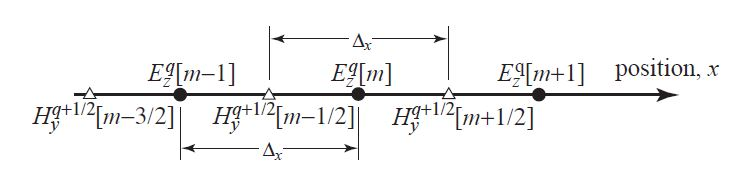
\includegraphics[width=4in]{Pictures/1dfdtd.jpg}
		%\rule{35em}{0.5pt}
	\caption[1 dimensional FDTD Space]{A one-dimensional FDTD space showing the spatial offset between magnetic and electric fields.}
	\label{fig:1dfdtd}
\end{figure} 

%-----------------------------------
%	SUBSECTION 1.3
%-----------------------------------
\subsection{One-Dimensional FDTD simulation}
To simulate  equations \eqref{eq:mag} and \eqref{eq:ele} in MATLAB we have to keep in mind following things:
MATLAB uses integer numbers for indexes of arrays hence we use does not set an offset of $\frac{1}{2}$ instead we use same integers for indexes as well, Figure \ref{fig:fdtdpc} shows a graphical representation of FDTD algorithm with integer indexes
\begin{figure}[htbp]
	\centering
		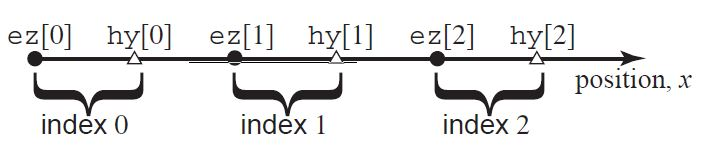
\includegraphics[width=5in]{Pictures/fdtdpc.jpg}
		%\rule{35em}{0.5pt}
	\caption[1 dimensional FDTD Space assumed with integer indices]{A one-dimensional FDTD space showing the assumed indexes and locations of magnetic and electric component in spatial domain}
	\label{fig:fdtdpc}
\end{figure}
Keeping figure \ref{fig:fdtdpc} in mind, the two update equations become
\lstset{language=Matlab, commentstyle=\color{green!50!black}, keywordstyle=\color{blue}, stringstyle=\color{red!60!black}}
\begin{lstlisting}
for m=0:SIZE-1
	hy[m] = hy[m] + (ez[m + 1] - ez[m]) / imp0;
end
for m=1:SIZE
	ez[m] = ez[m] + (hy[m] - hy[m - 1])  * imp0;
end
\end{lstlisting}
where imp0 is impedance of free space.
The reason behind different loop start and end point is that at end nodes there are no neighboring nodes to one side. For example hy[-1] node for ez[0].
As the field is initially zero it will remain zero as there is no energy passing through it. to overcome this problem a source node is hard-coded into one of the entry of array 
\lstset{language=Matlab, commentstyle=\color{green!50!black}, keywordstyle=\color{blue}, stringstyle=\color{red!60!black}}
\begin{lstlisting}
	ez(1) = exp(-(qTime - 30) * (qTime - 30) / 100.); %update node hard-coded
\end{lstlisting}

\textbf{Results}\\
By using the program in Appendix %ref here
we get the results in figure \ref{fig:fdtdpc}.
\begin{figure}[htbp]
	\centering
		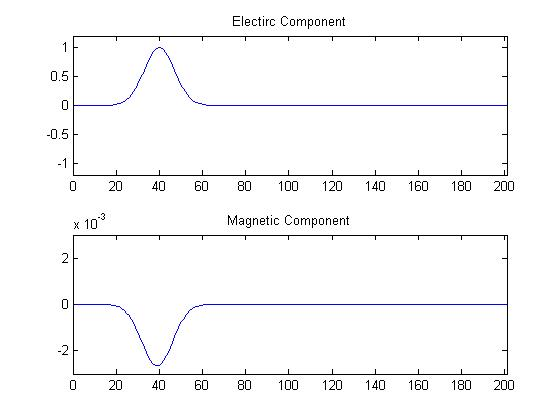
\includegraphics[width=5in]{Figures/free.jpg}
		%\rule{35em}{0.5pt}
	\caption[Simulation Result of 1 dimensional FDTD in free space]{Simulation Results of one-dimensional FDTD in free space showing both electric and magnetic component}
	\label{fig:fdtdpc}
\end{figure}
%-----------------------------------
%	SUBSECTION 1.4
%-----------------------------------
\subsection{Boundary Conditions}
Grid termination is called boundary condition because there are no neighboring values at boundary. we must use some kind of boundary condition depending upon the requirements. two type of boundary conditions are mentioned below.
%-----------------------------------
%	SUBSECTION 1.4.1
%-----------------------------------
\subsubsection{Perfect Conductor Boundary}
In program appendix % ref here
grid is terminated with a zero value of magnetic field
making it a perfect magnetic conductor (PMC) which reflects the wave completely. it also inverts the magnetic component of the wave figure \ref{fig:pmc}. In reality PMC does not exists hence to make this simulation as close to real behavior we use some other method to truncate the grid.
\begin{figure}[htbp]
	\centering
		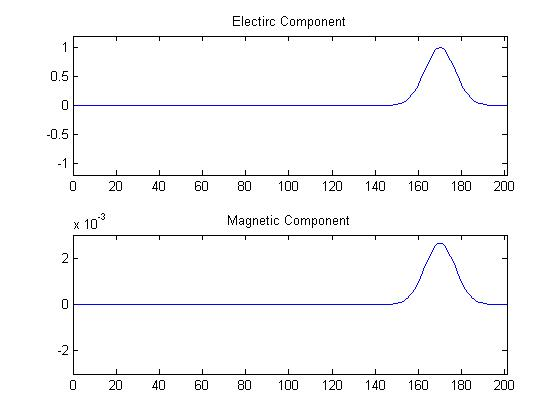
\includegraphics[width=5in]{Figures/pmc.jpg}
		%\rule{35em}{0.5pt}
	\caption[Simulation Result of 1 dimensional FDTD in free space with Perfect magnetic conductor boundary]{Simulation Results of one-dimensional FDTD after reflecting from Perfect magnetic conductor}
	\label{fig:pmc}
\end{figure}
%-----------------------------------
%	SUBSECTION 1.4.2
%-----------------------------------
\subsubsection{Absorbing Boundary Conditions}
Perfect conductor boundary depends on the speed of propagation. It requires that at each time instant the wave also propagate by one spatial step, but with the introduction of dielectric (slab) the speed of propagation decreases resulting in unstable simulation. hence we need an advance boundary condition which is differential equation based absorbing boundary condition (ABC).
\begin{equation}
	E_z^{q+1} \left[ 0 \right] = E_z^q \left[ 1 \right] + \frac {\frac{S_c}{\sqrt\mu_r\epsilon_r}-1} {\frac{S_c}{\sqrt\mu_r\epsilon_r}+1} \left( E_z^{q+1} \left[ 1 \right] - E_z^q \left[ 0 \right]  \right)
\label{abc}
\end{equation}
Equation \eqref(abc) is absorbing boundary equation %ref here
for electric field. As it can be seen that this boundary condition also depends upon last time step value at boundary point. so we need to save that value in our program as well.
Program in appendix %ref here
implements this boundary condition.

\textbf{Results}\\
Figure \ref{fig:abc} shows Gaussian wave after passing through a denser slab with absorbing boundary condition
\begin{figure}[htbp]
	\centering
		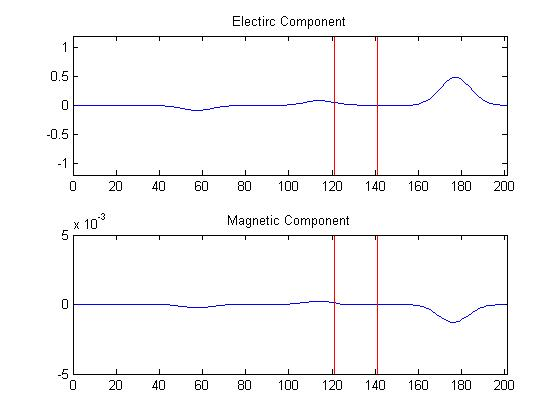
\includegraphics[width=5in]{Figures/abc.jpg}
		%\rule{35em}{0.5pt}
	\caption[Simulation Result of 1 dimensional FDTD after passing through denser medium]{Simulation Results of one-dimensional FDTD after passing through denser medium with absorbing boundary conditions}
	\label{fig:abc}
\end{figure}

%-----------------------------------
%	SUBSECTION 1.5
%-----------------------------------
\subsection{Simulation Results}
Following results were found after running program %ref here
 this program implements FDTD algorithm in free space, denser medium slab, additive source and absorbing boundary conditions.
%-----------------------------------
%	SUBSECTION 1.5.1
%-----------------------------------
\subsubsection{Simulation Parameters}
Parameters for program %ref here
are \\
Medium 1 = Free space  $\mu=\mu_0$  $\epsilon=\epsilon_0$\\
Medium 2 = slab of denser medium $\mu=2\mu_0$  $\epsilon=2\epsilon_0$\\
Courant Number $S_c=1$\\
Source type = Additive\\
Boundary conditions = Absorbing boundary conditions
%-----------------------------------
%	SUBSECTION 1.5.2
%-----------------------------------
\subsubsection{Frequency Domain Analysis}
Frequency domain analysis compares the theoretical values with that of simulated values.
 In Frequency domain analysis spectrum of transmitted and Incident waves are plotted. 
Refractive index is also calculated which should be equal to calculated refractive index given by equation \eqref{refractiveindex}
\begin{equation}
	\eta=\sqrt\epsilon_r\mu_r
\label{refractiveindex}
\end{equation}
for medium having $\mu=2\mu_0$  $\epsilon=2\epsilon_0$ result of equation \eqref{refractiveindex} comes out to be 1.414

\begin{figure}[htbp]
	\centering
		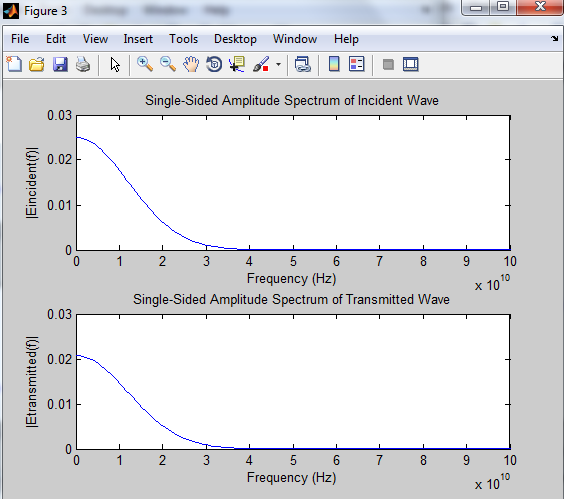
\includegraphics[width=5in]{Figures/fft1.png}
		%\rule{35em}{0.5pt}
	\caption[Frequency Spectrum of 1D denser medium slab]{Frequency Spectrum of transmitted and reflected wave after passing through a slab of denser medium having $\mu=2\mu_0$  $\epsilon=2\epsilon_0$ }
	\label{fig:fft1}
\end{figure}
\begin{figure}[htbp]
	\centering
		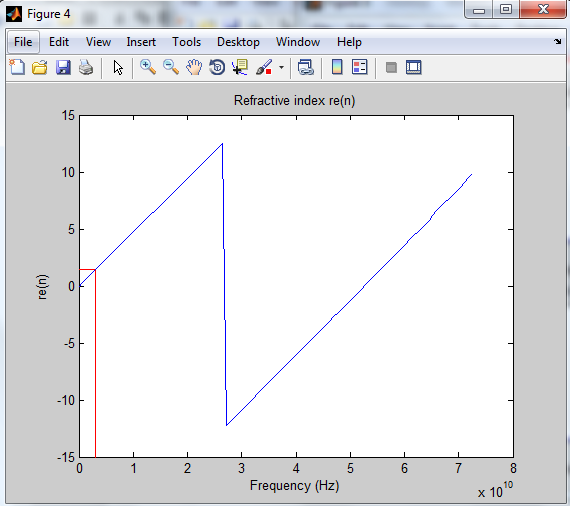
\includegraphics[width=5in]{Figures/ri1.png}
		%\rule{35em}{0.5pt}
	\caption[Refractive index of different frequencies after passing through denser medium]{Refractive index of different frequencies after passing through denser medium, Red lines shows the theoretical values of refractive index at 3Ghz Frequency}
	\label{fig:ri1}
\end{figure}
From figure \ref{fig:ri1} it is clear that simulation result and theoretical results are same as calculated from equation \eqref{refractiveindex}.
%-----------------------------------
%	SECTION 2
%-----------------------------------
\section{Modeling of NIM slab }
%-----------------------------------
%	SUBSECTION 2.1
%-----------------------------------
\subsection{Limitation of FDTD}
The standard FDTD does not work for negative values of permittivity and permeability. Reason behind this is Courant stability criterion. hence a NIM object can not be modeled using standard FDTD algorithm. Drude dispersive model or Lorentz model are used to implement NIM object. These models introduce frequency of operation $(\omega)$ into update equations.
%-----------------------------------
%	SUBSECTION 2.2
%-----------------------------------
\subsection{The Drudes Model}
Ideally permeability and permittivity of a material remain constant for all values of operating frequencies. However in reality Speed of electromagnetic waves changes with frequency and there is also loss due to particle collisions inside material. A material is called dispersive if it's permeability or permittivity is frequency dependent.
Paual Drude proposed a model of transport properties in materials in 1990\citep{drude}.
\begin{equation}
	M\frac{d^2x}{dt^2} = QE(t) - Mg\frac{dx}{dt}
\label{drudee1}
\end{equation}
Equation \eqref{drudee1} is a Drude's 2nd order differential equation that relates to kinetic energy in moving charges under an electric field. The relative Permittivity in Drudes model is given by 
\begin{equation}
\hat{\epsilon_r} (w) = \epsilon_{\infty}- \frac{\omega_p^2}{\omega^2 - jg\omega}
\label{drudee2}
\end{equation}
setting $g=0$ and $ \epsilon_{\infty} = 1$ in equation \eqref{drudee2}, value of permittivity comes out to be negative for $\frac{\omega}{\omega_p} > 1$ (figure \ref{drude1})
\begin{figure}[htbp]
	\centering
		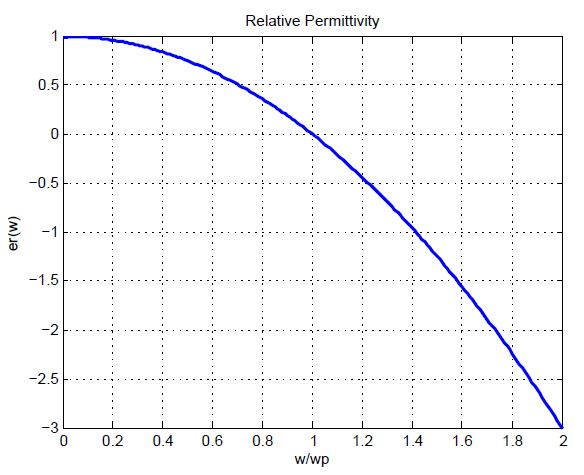
\includegraphics[width=5in]{Figures/drude1.jpg}
		%\rule{35em}{0.5pt}
	\caption[Permittivity in Drudes model for different frequencies]{Relative Permittivity plotted against $\frac{\omega}{\omega_p}$ for $g=0$ and $ \epsilon_{\infty} = 1$ }
	\label{drude1}
\end{figure}

%----------------------------------------------------------------------------------------
%	SUB SUB SECTION 2.2.1
%----------------------------------------------------------------------------------------

\subsubsection{Drudes Algorithm}
Auxiliary update equations for electric and magnetic components in Drudes model are give by \eqref{drudemag} and \eqref{drudeele}.
\begin{equation}
\begin{split}
	H_y^{n+1} &= a_m \left( B_y^{n+1} - 2B_y^n + B_y^{n-1} \right) + b_m \left( B_y^(n+1) - B_y^{n-1}  \right)\\
&+c_m \left( 2H_y^n-H_y^{n-1} \right) + d_m \left( 2H_y^n + H_y^{n-1} \right) +e_m H_y^{n-1}\\
\end{split}
\label{drudemag}
\end{equation}
\begin{equation}
\begin{split}
	E_z^{n+1} &= a_e \left( D_z^{n+1} - 2D_z^n + D_z^{n-1} \right) + b_e \left( D_z^(n+1) - D_z^{n-1}  \right)\\+ 
&c_e \left( 2E_z^n-E_z^{n-1} \right) + d_e \left( 2E_z^n + E_z^{n-1} \right) +e_e E_z^{n-1}
\label{drudeele}
\end{split}
\end{equation}
Update Equation for wave propagation in $-x$ direction are given by 
\begin{equation}
	B_y^{n+1}(k)=  B_y^{n} (k) + \frac {\Delta t}{\Delta z} \left( E_z^n (k) - E_z^n (k+1) \right)
\label{drudeby}
\end{equation}
\begin{equation}
	D_z^{n+1}(k)=  D_z^{n} (k) + \frac {\Delta t}{\Delta z} \left( H_y^n (k-1) - H_y^n (k) \right)
\label{drudedz}
\end{equation}

%-----------------------------------
%	SUBSECTION 2.3
%-----------------------------------
\subsection{Simulation of 1D DNG Slab}
%-----------------------------------
%	SUBSECTION 2.3.1
%-----------------------------------
\subsubsection{Problem Specification}
An EM wave is incident on a slab with negative permittivity and permeability ($\epsilon_r= -1$ $\mu_r= -1$) at frequency of 3Ghz for Sinusoidal wave. Gaussian wave is also applied to same slab for wide range frequency analysis. MATLAB code is available in 
Appendix %ref here
%-----------------------------------
%	SUBSECTION 2.3.2
%-----------------------------------
\subsubsection{Simulation Parameters}
Frequency of Operation $f=3 GHz$, $S_c=1$, in order to get $\epsilon_r= -1$ $\mu_r= -1$ plasma frequency needs to be $\omega_{pm}^2 = \omega_{pe}^2 = 2 \times (2\pi f_0)^2$ with $\epsilon_\infty = \mu_\infty = 1$.Absorbing Boundary Conditions are applied at field boundary.
%-----------------------------------
%	SUBSECTION 2.3.3
%-----------------------------------
\subsection{Simulation Results}
Following Results are obtained from simulation of 1D DNG slab.\\
\textbf{Gaussian Source}\\
Figure \ref{drude3} shows the snapshot of simulation after the Gaussian pulse entered the slab. it can clearly be seen that the wave is converted into different waveforms having different frequencies. It shows that dispersive material changes the speed of EM waves depending upon the value of $\epsilon \& \mu$.\\
Figure \ref{drude4} compares the theoretical value of refractive index with that of simulation results. As the slab under observation had a plasma frequency calculated at 3Ghz for $\epsilon_r= -1$ $\mu_r= -1$ the error is minimum around this frequency. Which proves that slab is acting as a NIM for 3GHz frequency of operation.
\begin{figure}[H]
	\centering
		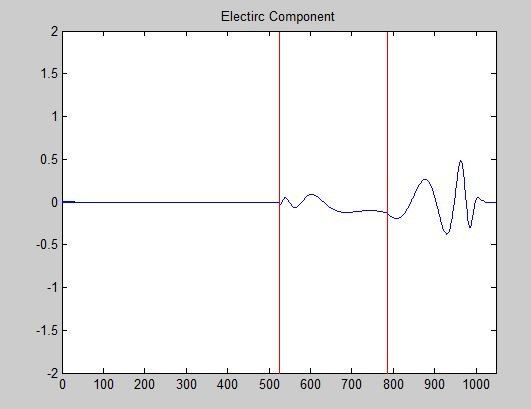
\includegraphics[width=5in]{Figures/drude3.jpg}
		%\rule{35em}{0.5pt}
	\caption[Gaussian Pulse after Passing through DNG slab]{conversion of Gaussian pulse into multiple wave forms of different frequencies after passing through dispersive DNG slab}
	\label{drude3}
\end{figure}

\begin{figure}[H]
	\centering
		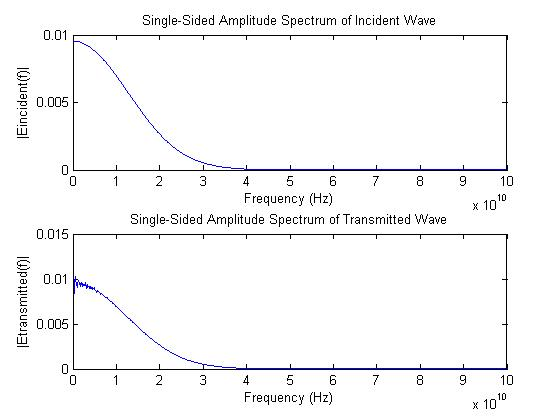
\includegraphics[width=5in]{Figures/drude5.jpg}
		%\rule{35em}{0.5pt}
	\caption[Reflected and Transmitted wave's Frequency Spectrum for 1D DNG simulation]{Reflected and Transmitted waves Frequency Spectrum for 1D DNG simulation with Gaussian wave as source}
	\label{drude5}
\end{figure}
\begin{figure}[H]
	\centering
		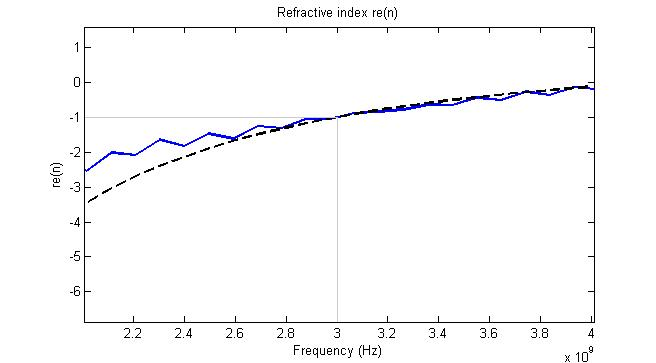
\includegraphics[width=5in]{Figures/drude4.jpg}
		%\rule{35em}{0.5pt}
	\caption[Refractive Index vs Frequency for 1D DNG slab]{Refractive indexes(Y-axis) Vs Frequency Graphs(X-axis) for 1D DNG slab, Black dashed line shows theoretical values, Blue line shows simulation results and calculated values, Grey lines mark the Frequency under study i.e 3GHz }
	\label{drude4}
\end{figure}
\textbf{Sinusoidal Source}\\
Figure \ref{drude2} shows the snapshot of simulation with Sinusoidal wave as source. it can be seen clearly that in steady state the wave entering the slab is identical to wave exiting the slab which implies that the reflected portion is approximately equal to zero. inside slab the wave seems to travel in opposite direction this is because the phase velocity\footnote{phase velocity of a wave is the rate at which the phase of the wave propagates in space} become negative inside NIM however the group velocity\footnote{group velocity of a wave is the velocity with which the overall shape of the waves' amplitudes ( known as the modulation or envelope of the wave) propagates through space.} is still in $-x$ direction.
\begin{figure}[H]
	\centering
		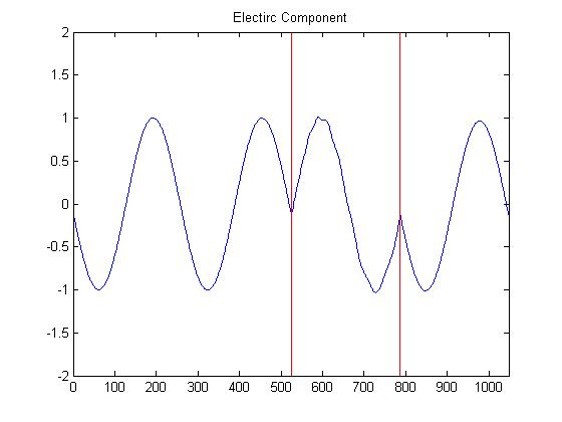
\includegraphics[width=5in]{Figures/drude2.jpg}
		%\rule{35em}{0.5pt}
	\caption[Sinusoidal wave passing through DNG slab]{Sinusoidal wave of 3Ghz passing through a slab of NIM}
	\label{drude2}
\end{figure}
%----------------------------------------------------------------------------------------
%	SECTION 3
%----------------------------------------------------------------------------------------

\section{Implementation in C++}

Before implementing the code on GPU it needs to be converted in c++ as OpenCL use c99 which is similar to C (more details of OpenCL in %ref here
). c++ have the basic functions to run the main loop, but it does not provide post processing utilities we require, natively, also graphical plotting is not supported. hence we must transfer the results of computation back to MATLAB for plotting and post processing.
%-----------------------------------
%	SUBSECTION 3.1
%-----------------------------------
\subsection{File handling in c++}
As our domain space can be very large the data produced by this computation is also very large. To transfer this data in MATLAB it have to be first written in files, but managing these files is also another issue. suppose we have a spatial domain of 2048, and time domain of 4084, it means there will be 2048 different values for each time step, as the simulation calculates both transmitted and refractive wave parameters total no of files become $2*Total_Time$ with each file having 2048 entries.
to cater this problem a dynamic file allocation scheme was written which saves the value for each time step in separate file and automatically name it accordingly.
\lstset{language=[ISO]C++, commentstyle=\color{green!50!black}, keywordstyle=\color{blue}, stringstyle=\color{red!60!black},caption=c++ file handling variables and Directory creation, label=cright1}
\begin{lstlisting}
// -------- Save to file Variables -------- 
	fstream snapshot;
	std::string filename ;
	std::stringstream stream;
	stream<<"results";
	CreateDirectory(stream.str().c_str(), NULL) ;		//create directory of results
\end{lstlisting}
this code \ref{cright1} creates a directory named results to store the files in current project directory. header file \emph{windows.h} is required for this command.
\lstset{language=[ISO]C++, commentstyle=\color{green!50!black}, keywordstyle=\color{blue}, stringstyle=\color{red!60!black},caption=c++ file handling using auto naming of file, label=cright2}
\begin{lstlisting}
// -------- Saving to file -------- 
	stream.str(std::string());   						// clear stringstream
	stream<<"./results/"<<"Efield"<<medium<<"_"<<qTime<<".jd";   		// concatenate
	filename = stream.str();		 					// copy string
	snapshot.open(filename, ios::out|ios::binary);
	for (mm = 0; mm < SIZE; mm++)
		snapshot.write((char *)&ez[mm],sizeof(double));
	snapshot.close();
\end{lstlisting}
Above code \ref{cright2} runs in the main time loop and saves values of Efield at every iteration. it automatically name the file according to medium and time instance. .jd is a file extension of own choice. Complete code can be found in Appendix %ref here

Post processing and simulation movie is done by using MATLAB. below is the code to read the files written by c++ program
\lstset{language=Matlab, commentstyle=\color{green!50!black}, keywordstyle=\color{blue}, stringstyle=\color{red!60!black},caption=Read files in MATLAB, label=matread}
\begin{lstlisting}
	filepath=fullfile(pwd, 'results'); %set files directory path, pwd gets the current directory path
	% in main Time loop
	fidp = fopen(strcat(filepath,'\Efield',int2str(medium),'_',int2str(j),'.jd'),'r','l');
	        if fidp==-1
           	 display('Error');
       	        return
        	end
\end{lstlisting}
the code \ref{matread}  reads the files or else generate Error. $j$ is the variable used for main timing loop. with addition to these Efield values other simulation parameters are also written on individual files these parameters include Etransmitted, Ereflected, Ez1, Ez2 and simulation parameters (delta, k0, z1,z2). complete MATLAB code can be found in Appendix %ref here
\clearpage
%----------------------------------- 
%	SECTION 4
%-----------------------------------
\section{Implementation on GPU }
Graphical Processing Unit or GPU is a computational device designed with a different architecture and different purpose. GPUs are Faster than CPUs because they have more number of cores (up-to 512 on a single chip \cite{cpuvsgpunotes}
) as compared to CPU and they use techniques like pipelining \cite{ref:gpu2}. GPUs memory is faster due to a larger bus width. simulations on GPU are 10-30 times faster than CPU \cite{Ref:gpuvscpui}
. Hence the FDTD algorithm is implemented on GPU because it can be parallelized.

%-----------------------------------
%	SUBSECTION 4.2
%-----------------------------------
\subsection{OpenCL}
OpenCL (Open Computing Language) is a framework by KHRONOS Group %ref here
for parallel programming on heterogeneous systems. its main advantage is program portability, the same code can run on multiple devices such as CPU, GPU, FPGA, DSP kit \cite{ref:devices}
 etc. OpenCL framework include support for c++ however main kernels are written in language c99 which is a old standard for c language.
%-----------------------------------
%	SUBSECTION 4.3
%-----------------------------------
\subsection {OpenCL Program Flow}
To write a program in OpenCL we need to take care of Host side program, Kernel program, host side memory and device memory. the host is programmed in C/C++ while device is programmed using OpenCL C (c99).

\subsubsection{Kernel}
every function which runs on device is required to be in a kernel function

\lstset{language=C,caption=OpenCL Kernel function, label=kernel}
\begin{lstlisting}
__kernel void hy_kernel(__global PRECISION *hy, __global PRECISION *ez, __global PRECISION *mu, const PRECISION delt, const PRECISION delx, const int SIZE) 
{
	unsigned int i = get_global_id(0);
  if(i < SIZE)
    hy[i] = hy[i] + (ez[i+1] - ez[i]) * (delt/(delx*mu[i]));
}
\end{lstlisting}
OpenCl automatically manages \lstinline{global_id} and run them in parallel hence the multiplication result of  \lstinline{hy[i] = hy[i] + (ez[i+1] - ez[i]) * (delt/(delx*mu[i]));} are obtained simultaneously over the whole space.
\lstinline{__global PRECISION *hy} is used to pass an array into device memory. The kernel is only allowed read/write access to global, constant, local, and private memory, which is specified by \lstinline{ __global, __constant, __local, __private}, respectively.

\subsubsection{Host Program}
\label{HostProgram}
Host program executes the kernels using the API of OpenCL. Before running any program it initializes some parameters. In a complete run it performs a number of operations. which are listed below \cite{openclpro}.
\begin{enumerate}
\item Listing available platforms
\item Displaying platforms and get input for desired platform
\item Creating context
\item Creating command queue
\item Creating memory objects
\item Reading kernel file
\item Creation of program object
\item Compilation of kernel
\item Creating kernel object
\item Set kernel argument
\item Executing kernel
\item reading memory object
\item Releasing kernel
\item De-allocating memory in device
\end{enumerate}
\begin{figure}[H]
	\centering
		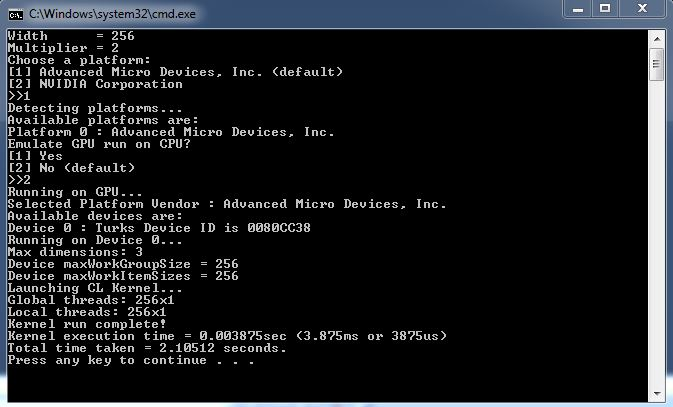
\includegraphics[width=6in]{Figures/opencl.jpg}
		%\rule{35em}{0.5pt}
	\caption[OpenCL basic run]{ Basics tasks performed by OpenCL API}
	\label{opencl}
\end{figure}

Complete codes can be found in Appendix %ref here
. After simulation post processing is done in MATLAB
%-----------------------------------
%	SUBSECTION 4.4
%-----------------------------------
\subsection {Challenges in GPU programming}
Main challenges in writing OpenCL program were

\subsubsection{Read Delay}
When data is passed to GPU or values are read from device memory to host memory considerable time is consumed. as in algorithm for boundary conditions we need pervious time step values so there were a lot of data transfer from host to device and device to host memory, and to save the values of Electric field arrays they need to be brought into host memory. to reduce the overhead time absorbing boundary condition was moved into kernal number 2, and snapshot (writing to file) interval was changed from each iteration to every 20th iteration \ref{kernel2}.
\lstset{language=C,caption=OpenCL saving Efield values in files, label=kernel2}
\begin{lstlisting}
if (qTime % 20 ==0) // Snapshot interval
{
      //// Copy data back to host ////
      SafeCall(clEnqueueReadBuffer(commandQueue, ez_gpu, CL_TRUE, 0,  sizeof(PRECISION)*SIZE, ez, 0, NULL, NULL), "Error reading ez back to host memory");    
      SafeCall(clWaitForEvents(1, &events[0]), "Error: Waiting for kernel run to finish. (clWaitForEvents)");
         // -------- Saving to file -------- 
			stream.str(std::string());   						// clear stringstream
			stream<<"./results/"<<"Efield"<<medium<<"_"<<qTime+1<<".jd";   		// concatenate
			filename = stream.str();		 					// copy string
			snapshot.open(filename.c_str(), ios::out|ios::binary);
			for (mm = 0; mm < SIZE; mm++)
			snapshot.write((char *)&ez[mm],sizeof(float));
			snapshot.close();
 } 
\end{lstlisting}

\subsubsection{Kernel syncronization}
As value of electric node depends on neghoboring magnetic field nodes and value of magnetic field nodes  depends on neghoboring elctric field nodes it is essential that all kernels run in a syncronized way, or else wrong values would be calculated because of inavailability of updated nodes values. becase all kernels are not performing same calculations it is prone to desyncronization. to run these kernel in syncronized method following command \ref{kernel3}  is used inside kernel 2. this command basically look for global (other) kernel speed ad it's local speed, then it adds a delay to syncronize it perfectly with other kernels. there is a tradeoff with this method which is extra computational time in which the kernel is just waiting for others to complete.
\lstset{language=C,caption=Kernel syncronization, label=kernel3}
\begin{lstlisting}
	barrier(CLK_GLOBAL_MEM_FENCE|CLK_LOCAL_MEM_FENCE);
\end{lstlisting}











